\documentclass{article}

% The LaTeX-to-CNXML translator makes use of Tralics, a LaTeX-to-XML conversion
% utility.  Tralics has implemented all the packages in the LaTeX base directory,
% and it also supports a good number of supplemental LaTeX packages.  These
% supplemental packages are included in the \usepackage{} statements below.
% Packages not in the LaTeX base directory or \usepackage{} statements in this
% template are not supported by Tralics and, hence, not supported by the
% LaTeX-to-CNXML converter.

% If you have a question as to whether a specific LaTeX command is supported,
% please refer to the "HTML Documentation of all TeX commands" section at
% http://www-sop.inria.fr/apics/tralics/.  Here you will find links to manual pages
% organized alphabetically by the first letter of the command.  These pages indicate
% how Tralics handles conversion of each supported command, which informs how the
% LaTeX-to-CNXML translator behaves.

% To prepare your LaTeX document for import, copy the body of that document from its
% source and paste it into this template between the \begin{document} and \end{document}
% statements.  Do not attempt to use any packages other than the ones contained in this
% template.  You may, however, insert user-defined macros directly in this template
% before the \begin{document} statement.  Following this preparation, check to see if
% your template-compliant document can generate a .dvi (.pdf) using latex (pdflatex).
% If so, then your document is ready for import; if not, you must modify your document
% to generate an output file using only the packages supported by Tralics as described
% above.

% Tralics supports the following AMS packages
% (see http://www-sop.inria.fr/apics/tralics/packages.html for details on full/partial
% support of package commands)
\usepackage{amsbsy,amscd,amsfonts,amsgen,amsmath,amsopn,amssymb,amstext,amsthm,amsxtra}

% Tralics supports \includegraphics and \scalebox, but not all other graphicx package
% commands; check the web documentation on supported commands before attempting to use
% other commands in the graphicx package:
\usepackage{graphicx}

% We must specifically invoke the verbatim package as follows to direct Tralics to handle
% the verbatim environment properly:
\usepackage{verbatim}

% Tralics also allows the following packages:
% (see http://www-sop.inria.fr/apics/tralics/packages.html for details on full/partial
% support of package commands)

%\usepackage{alltt}
%\usepackage{array}
%\usepackage{bracket}
%\usepackage{calc}
%\usepackage{delarray}
%\usepackage{eucal}
%\usepackage{eufrak}
%\usepackage{fancyverb}
%\usepackage{fix-cm}
%\usepackage{fixltx2e}
%\usepackage{flafter}
%\usepackage{fontenc}
%\usepackage{fp}
%\usepackage{graphpap}
%\usepackage{html}
%\usepackage{ifthen}
%\usepackage{index}
%\usepackage{inputenc}
\usepackage{latexsym}
%\usepackage{lipsum}
%\usepackage{makeidx}
%\usepackage{minimal}
%\usepackage{mml}
%\usepackage{natbib}
%\usepackage{newlfont}
%\usepackage{oldlfont}
%\usepackage{shortvrb}
%\usepackage{showidx}
%\usepackage{soul}
%\usepackage{syntonly}
%\usepackage{textcase}
%\usepackage{textcomp}
%\usepackage{tloop}
%\usepackage{theorem}
%\usepackage{upref}

%-------------------------------------------------------------------
% You can insert user-defined macros (using the supported packages
% only) here...
\providecommand{\abs}[1]{\left|#1\right|} 
\providecommand{\norm}[1]{\left|#1\right|} 
%-------------------------------------------------------------------

%INSERT FIGURE TEMPLATE
%\begin{figure}
%\begin{center}
%\includegraphics[scale=1]{filename}
%\caption{text}
%\label{fig:name}
%\end{center}
%\end{figure}

\begin{document}

%-------------------------------------------------------------------
% Begin entering your LaTeX document content here...
%\tableofcontents
\section{Background: Place Cells in the Hippocampus}
\subsection{Biology}
Spatial memory is what allows us to keep track of our location in space by making mental maps of each environment. Let's consider what happens in the brain during the process of forming these internal maps.

Connections, called synapses, between certain neurons strengthen or weaken--a process known as synaptic plasticity. The strength, or weight, of a synapse controls how much one neuron can affect another. Synaptic plasticity is necessary for memory formation \cite{Moser}.

While many neurons are involved with spatial memory, our focus is upon neurons in the hippocampus called place cells \cite{Moser}. Place cells have a unique firing pattern. When an environment becomes familiar, each place cell becomes associated with one area of the environment. In other words, after repeated exposure to one environment, a place cell will come to spike in only one area of the environment, which is called that cell's place field \cite{Moser}. See Figure \ref{fig:placefield}.

%INSERT FIGURE
\begin{figure}
\begin{center}
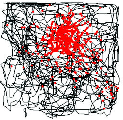
\includegraphics[scale=1]{Moser-Placefield}
\caption{The place field of one place cell. As a rat explored the square environment, experimenters monitored the activity of one place cell.�The black line is the rat's trajectory, and each red dot represents a location that the place cell has become active. The place field of the particular place cell that was monitored is the area of the environment marked densely by red dots \cite{Moser}.} \label{fig:placefield}
\end{center}
\end{figure}

Due to place cells' characteristic firing pattern where a cell has a single place field in each environment, it is easy to test if a rat recognizes the environment they have been placed in by examining place cell activity.

\subsection{Motivation: Double Rotation Experiment}
Our research on place cells is based off of the Double Rotation Experiment (DRE) conducted by our collaborator Dr. Knierim \cite{KnierimDRE}. 

%INSERT FIGURE of DR experiment
\begin{figure}
\begin{center}
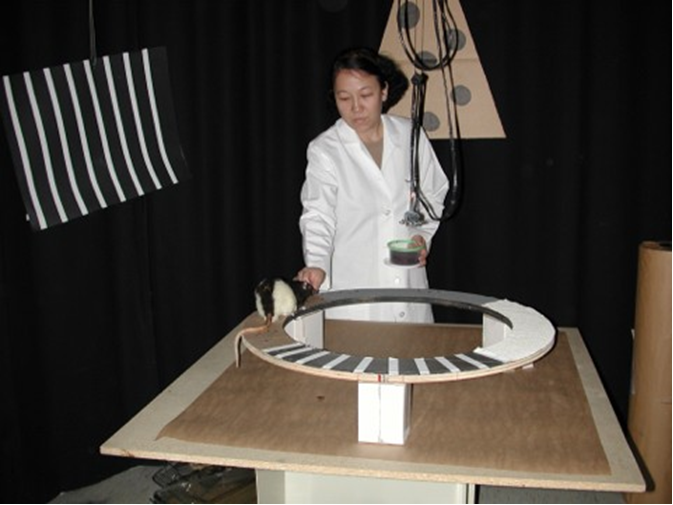
\includegraphics[scale=0.5]{doublerotationReal}
\caption{The Double Rotation Experiment (DRE). Rats were trained to walk clockwise around the track, and the place fields corresponding to specific locations on the track were monitored. During the learning phase, the place fields experienced a backward shift. During double rotation runs of the experiment, the local cues were rotated backward (counterclockwise), and the place fields shifted backward as well. Thus the place fields seemed to favor following the local cues. Perhaps the natural backward shift seen in the learning phase predisposes the place fields to wanting to follow cues that move backwards \cite{KnierimDRE}.} 
\label{fig:DRE}
\end{center}
\end{figure}
 
His team set up a track that a rat traversed and monitored the place fields that corresponded to specific locations on the track. Dr. Knierim and his team set up local cues on a circular path and distal cues on surrounding curtains and trained rats to walk along the path in a clockwise direction. The place fields corresponding to specific locations on the track were monitored. See Figure \ref{fig:DRE}.

During the learning phase, as the rat completed laps and became more familiar with the layout, the place fields shifted backward along the path opposite the rat's movement. 
In standard runs of the experiment, the rat ran clockwise around the path with the layout that it learned. In double rotation runs of the experiment, the local cues were rotated counterclockwise (backward) and distal cues were rotated in clockwise--hence the ``double rotation". 
During the standard and the double rotation runs, the spatial inputs and place fields did not always match. In the double rotation runs, the spatial inputs tended to follow the distal cues, whereas the place fields tended to follow local cues. 

One thing that might explain this is the backward shift seen in the learning phase. The natural backward shift of place fields that happens when a rat has become familiar with its environment appears to bias the place fields to follow the cues that shift backwards. The backward shift of place fields has been observed in other experiments as well when rats became familiar with a path \cite{Mehta}. It may be that the backward shift is a part of the learning process. Thus, we want to understand more about the backward shift and aim our research in this direction.

The backward shift may be dependent upon the weights of synapses, yet the dependence is not well understood. We focus on how the dynamic weights due to synaptic plasticity affect the backward shift of place fields.

We implemented a far simplified model of the DRE to try to understand this relationship better.

\section{Modeling}
\label{seq:modeling}
Here we will describe the models used throughout the summer. A circuit model allows us to understand the mechanics of one neuron, while a 120-cell ring models the Double Rotation Experiment \cite{KnierimDRE}, and a single-cell model was used for the analysis of weights and backward shift. Refer to Table \ref{tbl:param} for the parameters used throughout the models and their values.

\begin{table}
\begin{center}
\begin{tabular}{| c | c | c | }
\hline
Parameter & Value & Description\\ \hline
$w_{inp}$ & $2\leq w_{inp}\leq 20$ mV & Input weight\\
$I$ & $2\leq I\leq 30$ ms & Interspike interval of external inputs\\
$\tau$ & 20 ms & Decay time\\
$dt$ & 1 ms & Time step\\
$v_r $& -70 mV & Resting voltage\\ 
$v_{th}$ & -54 mV & Threshold voltage\\  \hline
\end{tabular}
\end{center}
\caption{Parameters for models. These values are used unless otherwise specified.}
\label{tbl:param}
\end{table}

\subsection{Neuron as a Circuit: Integrate and Fire}

We model a single place cell with the Integrate and Fire (IAF) model so that we can accurately calculate the subthreshold voltage and approximate spike times of a cell at little computational expense \cite{Katie}.

\begin{figure}
\begin{center}
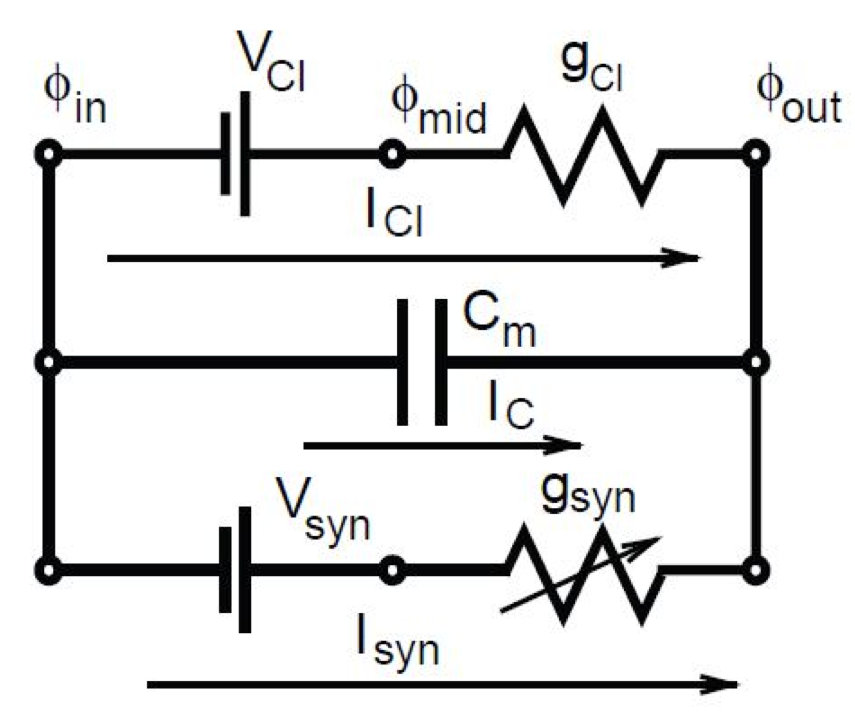
\includegraphics[scale=0.5]{Circuit}
\caption{Circuit model of a cell. The cell can be modeled as a circuit with three currents. The difference between potentials $\phi_{in}$ and $\phi_{out}$ gives the reversal potential $v_{Cl}$, which we refer to as $v$ in the text. $g_{Cl}$ and $g_{syn}$ denote the conductances of the chloride channels and the synapse, respectively. $C_m$ is the membrane capacitance. $v_{syn}$ depends upon the equilibrium concentrations of the ion of the associated channel. By Kirchoff's current law, $I_{Cl}+I_C+I_{syn}=0$, \cite{Cox}.} 
\label{fig:circuit}
\end{center}
\end{figure}

The cell can be modeled as a leaky capacitor that separates charge by controlling the flow of ions across the cell membrane, making a difference between potentials $\phi_{in}$ and $\phi_{out}$ across the membrane ($v=\phi_{in}-\phi_{out}$). This model approximates the subthreshold voltage ($v$ before it reaches the threshold voltage $v_{th}$) and the time that $v$ does reach threshold $v_{th}$. When $v$ reaches the threshold voltage, $v$ experiences a sharp increase then decrease and the cell is said to have ``spiked" or ``fired". 

Let $C_m$ denote the membrane capacitance, $g_{Cl}$ and $g_{syn}$ denote the conductances of the chloride channels and the synapse, respectively, and $v_{Cl}$ denote the reversal potential (the voltage at which no net flow of chloride ions occurs). $v_{syn}$ is determined by the equilibrium concentrations of the ion of the associated channel, \cite{Cox}. Input from other cells adds excitatory synaptic current. This input allows for the cell to depolarize and eventually reach $v_{th}$ and fire, which sends an electric signal to neighboring cells. The electric signal from a neighboring cell allows for voltage-gated channels to open, which affects the synaptic conductance $g_{syn}$. We set the reversal potential above a threshold voltage so that as $g_{syn}$ increases and the channels open, the cell's voltage $v$ approaches the threshold $v_{th}$. When $v\geq v_{th}$, the cell fires \cite{Cox}. See Figure \ref{fig:circuit} for a model of a cell as a circuit \cite{Cox}. 
The synaptic conductance is governed by the ODE
\begin{equation}
\tau g_{syn}'=-g_{syn}+\sum_i w_i^{inp}\sum_n \delta(t-T_n),  
\label{eq:cond}
\end{equation}
where $\tau$ is the decay constant, $w_i^{inp}$ is the weight of synaptic input from the $i$th synapse, $T_n$ is the set of input spike times for the presynaptic cell $i$, and $\delta$ is the Dirac delta function. From Dr. Cox's book \cite{Cox}, we see that applying Kirchoff's current law results in
\begin{equation}
C_m \frac{dv}{dt} + g_{Cl}(v-v_{Cl}) + g_{syn}(v-v_{syn})=0.
\label{eq:circuitvolt}
\end{equation}

\begin{figure}
\begin{center}
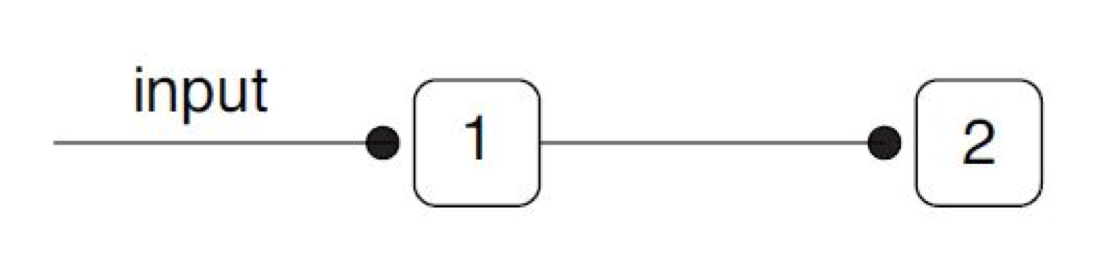
\includegraphics[scale=0.4]{model2cell}
\caption{Simple 2-cell network. Cell 1 receives input from an external source, and Cell 2 receives input from Cell 1. The conductances and voltages of the two cells are calculated by equations \eqref{eq:cond} and \eqref{eq:circuitvolt}, respectively \cite{Cox}.} 
\label{fig:2cellmodel}
\end{center}
\end{figure}

\subsection{Model of DRE: 120-cell Ring}
\label{seq:DRE}
\begin{figure}
\begin{center}
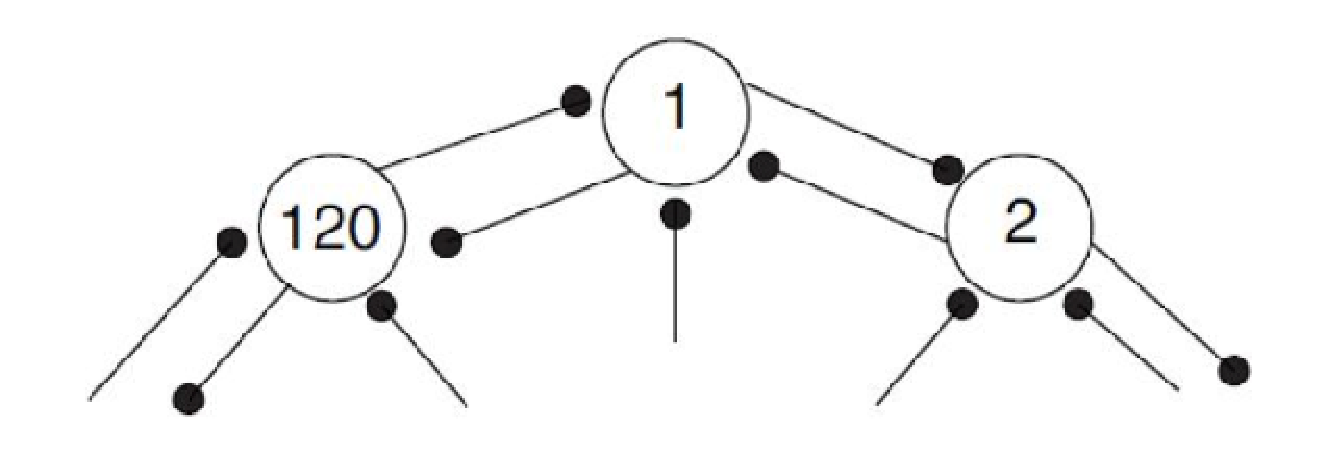
\includegraphics[scale=0.5]{ring120cell}
\caption{120-cell ring. We put 120 cells, represented by circles, in a ring architecture with bidirectional interactions between cells, as well as synapses to sources of external input.�Like the DRE, each place cell has a corresponding place field on a circular path that a simulated rat traverses clockwise. The bidirectional interaction between two neighboring cells is modeled through two synapses with one synapse for each direction \cite{Cox}. The weights of the synapses changes over time according to the STDP model described in Section \ref{seq:STDP} \cite{KnierimSTDP}.}
\label{fig:120cellring}
\end{center}
\end{figure}

We use the IAF model for single cells, and we connect these cells into a ring of 120 place cells to simulate the DRE \cite{Cox}.
The 120-cell ring is depicted in Figure \ref{fig:120cellring}. Each cell receives external spatial input as well as input from neighboring cells. The conductances and voltages of Cells 1 and 2 are depicted in Figure \ref{fig:IAFmodel} as calculated by equations \eqref{eq:cond} and \eqref{eq:circuitvolt}. We monitor the weights of the connections between neighboring cells over time, where there is an arbitrary maximum weight bound so that the weights do not approach infinity and a minimum weight bound of $0$ so the weights do not become negative. We also monitor how the changes of the weights affect the position of the place fields. See Figure \ref{fig:IAFmodel} for a depiction of the IAF model.

\begin{figure} 
\begin{center}
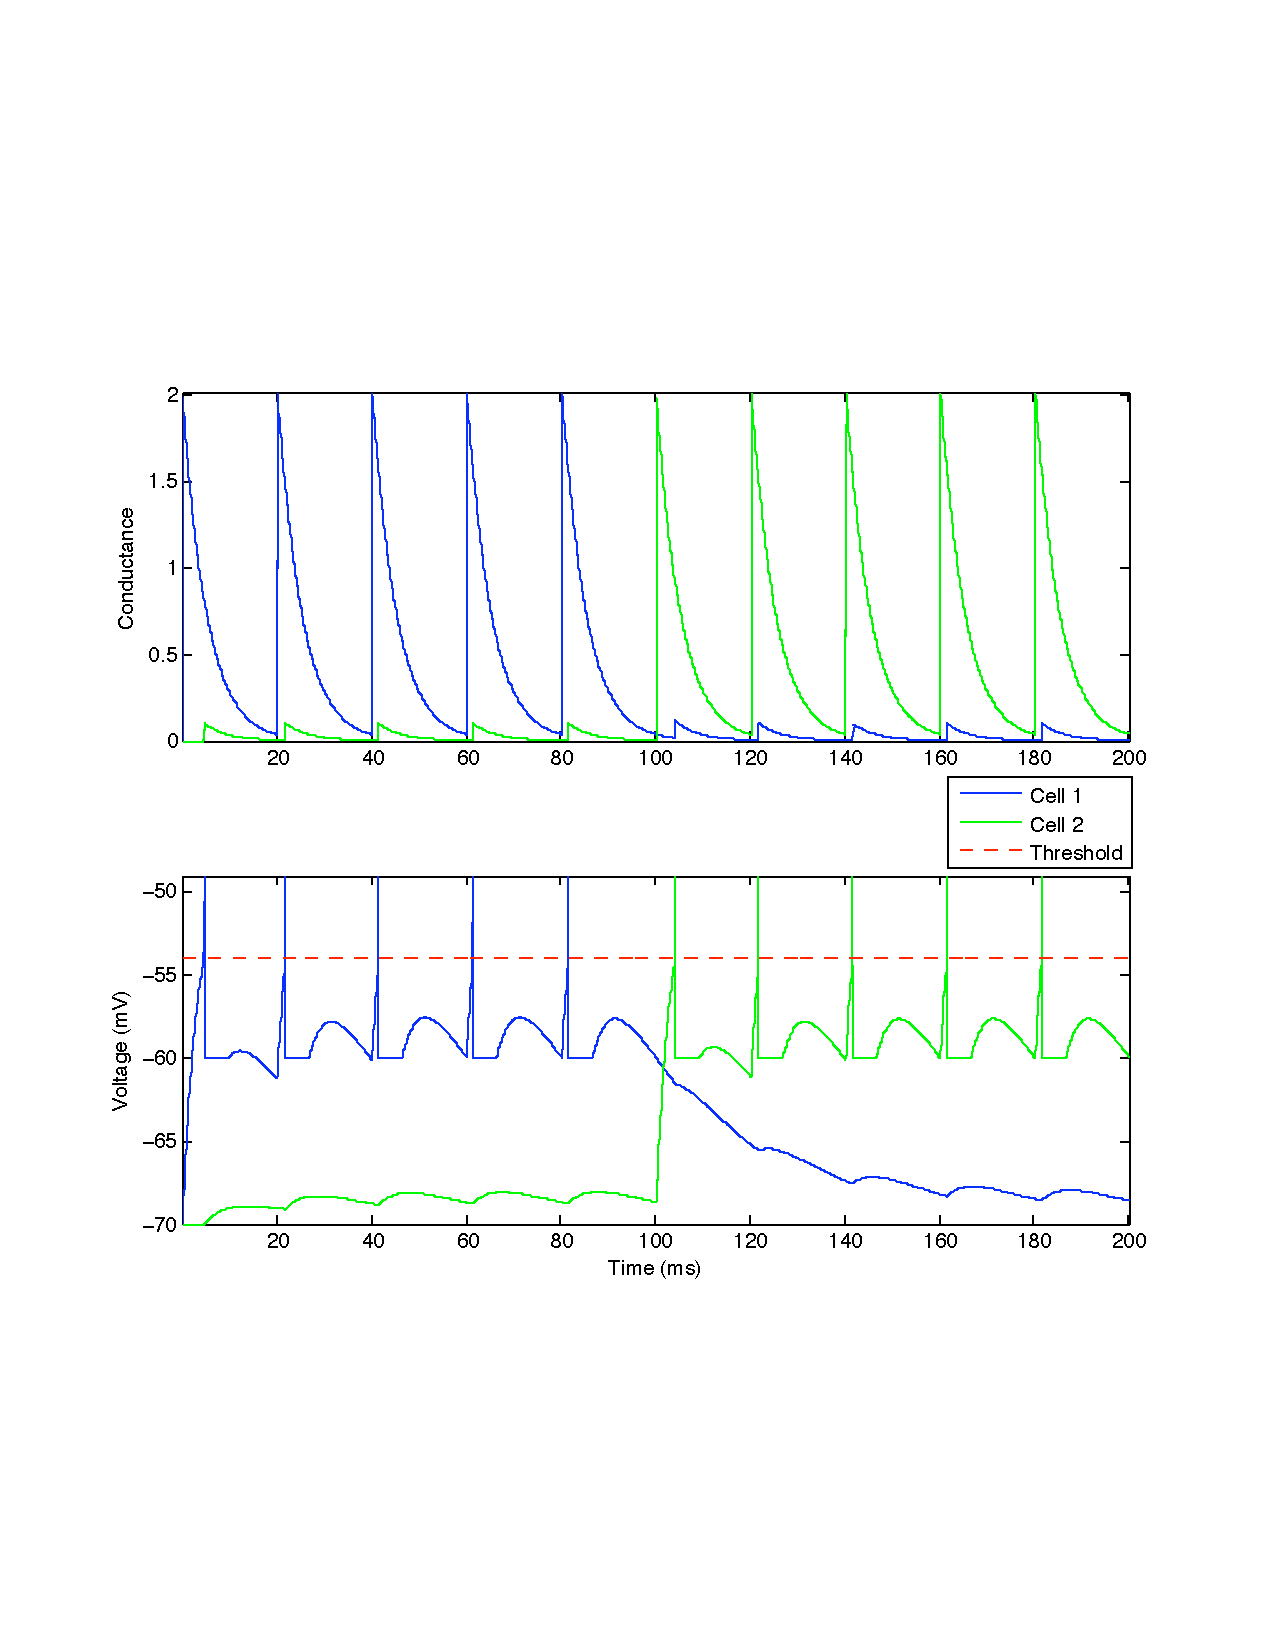
\includegraphics[scale=0.6]{IAF2cells}
\caption{Depiction of the IAF model for Cell 1 and Cell 2 from Figure \ref{fig:120cellring}. We calculate the conductances and voltages for Cells 1 and 2 by \eqref{eq:cond} and \eqref{eq:circuitvolt}, respectively. $v_{th}=-54\ mV$, and $w_{ext}=w_{12}=2\ S$ are the weights of the synapses from the external source and Cell 1, respectively. It can be seen that in Place Field 1 ($0<t<100$), Cell 1 receives external input every $20$ ms (in the form of conductance spikes), and in Place Field 2 ($100\leq t <200$), Cell 2 receives the external input. At each external input spike, the corresponding cell fires (its voltage spikes) and gives a small amount of input to its neighboring cells. (\textbf{IAF2cellsweight.m})} 
\label{fig:IAFmodel}
\end{center}
\end{figure}

\subsubsection{STDP}
\label{seq:STDP}
To determine how the weights of the synapses change, we use an STDP model \cite{KnierimSTDP}.
The spikes times of the pre- and post-synaptic cells are compared, and the smaller the time difference, the more the weight is adjusted. See Figure \ref{fig:STDP}. The percentage of weight change is determined by
\begin{equation}
F(\Delta t) = \left\{
\begin{array}{ll}
A_+ e^{\Delta t /\tau_+}, & \Delta t<0\\
-A_- e^{-\Delta t/\tau_-}, & \Delta t\geq 0,
\end{array} \right.
\label{eq:STDP}
\end{equation}
where $\Delta t=t_{pre}-t_{post}$ and $A_+$ and $A_-$ scale the maximal amount of change allowed when $\Delta t$ is close to $0$ \cite{KnierimSTDP}. $F(\Delta t)$ is depicted in Figure \ref{fig:STDP}.

\begin{figure}
\begin{center}
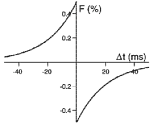
\includegraphics[scale=1]{STDPweightchange}
\caption{Percentage of weight change due to STDP. This graph shows that as $\Delta t=t_{pre}-t_{post}$ approaches $0$, the percentage of change in the weight of the synapse increases \cite{KnierimSTDP}. $F(\Delta t)$ is calculated by Equation \ref{eq:STDP}.} 
\label{fig:STDP} 
\end{center}
\end{figure}

In our 120-cell model, we set a lower bound for the weights at $0\ mV$ and an upper bound at $5\ mV$. The necessity for an upper weight bound is one of the weaknesses of the STDP model, so Andrew Wu, another member of this PFUG, has done work with other plasticity models. See his work [here]. %refer to Andrew

The work with the 120-cell model is all computational. Our results show that each lap, the weight of the synapse from Cell 1 to Cell 2 ($w_{12}$) increases toward a set weight bound and the weight of the synapse from Cell 2 to Cell 1 ($w_{21}$) decreases to 0 as in Figure \ref{fig:STDPweights}. We also see that after $4$ laps around the path, the place fields start to shift backward. Figure \ref{fig:STDPtime} shows that the spike time of Cell 2 decreases each lap, which is indicative of a backward shift of Cell 2's place field. See \textbf{IAF120cells1stspks.m}. 

\begin{figure}
\begin{center}
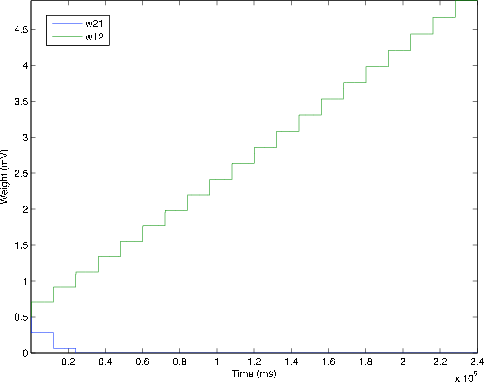
\includegraphics[scale=0.65]{STDPweights}
\caption{Weights of synapses over time. The weight of the synapse from Cell 1 to Cell 2 ($w_{12}$) increases each lap (1 lap = 12,000 ms) as the weight of the synapse from Cell 2 to Cell 1 ($w_{21}$) decreases each lap to 0. (\textbf{IAF120cellsSTDP.m})} 
\label{fig:STDPweights} 
\end{center}
\end{figure}

\begin{figure}
\begin{center}
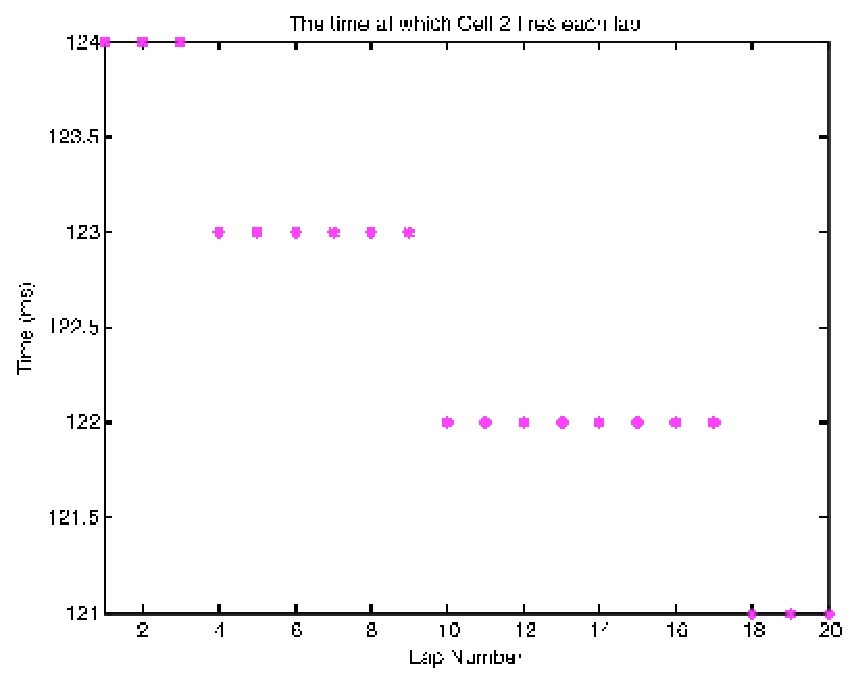
\includegraphics[scale=0.75]{IAF120cells1stspks}
\caption{Backward shift of place field of Cell 2 in $ms$. The rat spends $100\ ms$ in each place field. It can be seen here that after as few as $4$ laps around the track, place cell $2$ starts to fire earlier and its place field shifts backwards. (\textbf{IAF120cells1stspks.m})} 
\label{fig:STDPtime} 
\end{center}
\end{figure}


\subsection{Model for Analysis}
\begin{figure}
\begin{center}
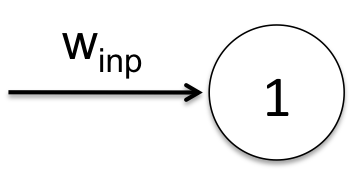
\includegraphics[scale=0.75]{model1cell}
\caption{Simple 1-cell system. Cell 1 receives input of weight $w_{inp}$ at an interspike interval $I$.} 
\label{fig:1cellmodel} 
\end{center}
\end{figure}

We begin by considering only one place cell which receives input from one external source with constant weight $w_{inp}$ at a set interspike interval, $I$, as depicted in Figure \ref{fig:1cellmodel}. The following equation gives the voltage $v$ in $mV$ of the cell at time $t$ with $n$ total input spikes:
\begin{equation}
\label{eq:vmodel}
\tau v'(t) = (v_r - v(t)) + w_{inp}\sum_{i=1}^n\delta(t-T_i)
\end{equation}
where $\tau=20$ $ms$ is the membrane time constant, $v_r=-70$ $mV$ is the resting potential,  $T$ is the set of input spike times, and $\delta(t-T_i)$ is the Dirac delta function. This is a simplification of equation \eqref{eq:circuitvolt}.

\subsubsection{Computational Method}
To solve for $v(t)$ computationally, we first look at the times with no input spikes ($kI<t<(k+1)I$).
Integrating both sides of equation \eqref{eq:vmodel} from $t-dt$ to $t$ and using the trapezoid rule, we find
\begin{align}
\tau(v(t)-v(t-dt)) &= v_r dt - \frac{v(t)+v(t-dt)}{2},\quad\text{which can be rearranged as} \notag\\
v(t) &= \frac{2dt}{2\tau + 1}\cdot v_r + \frac{2\tau-1}{2\tau +1}\cdot v(t-dt). \label{eq:compvbtwn}
\end{align}

When there is an input spike, we add $w_{inp}$ to $v(t)$, which is shown in
\begin{equation}
v_{inp}(t) = v(t) + w_{inp}. \label{eq:compvinp}
\end{equation}


\subsubsection{Analytic Method}
To solve for $v(t)$ analytically, we first look at $v(t)$ between input spikes. From equation \eqref{eq:vmodel}, we get
$$\tau v'(t) = (v_r - v(t)).$$
Solving this ordinary differential equation gives us
$$v(t) = v_r + ce^{-t/\tau},$$
where $c$ is the constant of integration. We know we want $v(0)=v_r+w_{inp}$, so $c$ must equal $w_{inp}$. Thus, we have 
$$v(t) = v_r + w_{inp}e^{-t/\tau},\ \text{where}\ 0\leq t<I,$$
which simply tells us that after one input spike at $t=0$, $w_{inp}$ decays so that $v(t)$ approaches $v_r$. Consider the following calculations of $v(t)$ for up to three input spikes.

At $t=I$, we have a second input spike, and at $I<t<2I$, we decay the input to find
\begin{align*}
v(I\leq t<2I) &= v_r + w_{inp}e^{-t/\tau}+w_{inp}e^{-(t-I)/\tau}.
\end{align*}
Finally, at $t=2I$, we have a third input spike and see
$$v(2I) = v_r + w_{inp}e^{-2I/\tau}+w_{inp}e^{-I/\tau} + w_{inp}.$$

To determine when the voltage reaches threshold and the cell spikes, we need only examine the peak values of $v$,  which are when $t=kI, \ 0\leq k\leq n-1$. Thus, we use the following generalized formula to calculate $v((n-1)I)$ when there are $n$ total input spikes:
\begin{equation}
\label{eq:anvinp}
\forall n, \quad v((n-1)I) = v_r + w_{inp} \sum_{k=0}^{n-1} \left(e^{-I/\tau}\right)^{k}.
\end{equation}
Figure \ref{fig:AnpeakV} shows that in the absence of spikes, the peak voltages approach an asymptote. This asymptote can be calculated by
\begin{align}
v_\infty = \lim_{n\rightarrow\infty} v((n-1)I) &= v_r + w_{inp} \sum_{k=0}^{\infty} \left(e^{-I/\tau}\right)^k \notag\\
 &= v_r + w_{inp}\left(\frac{1}{1-e^{-I/\tau}}\right). \label{eq:Vasymp}
\end{align}
If $v_\infty<v_{th}$, then the cell will never spike.

\begin{figure}
\begin{center}
\label{fig:AnpeakV}
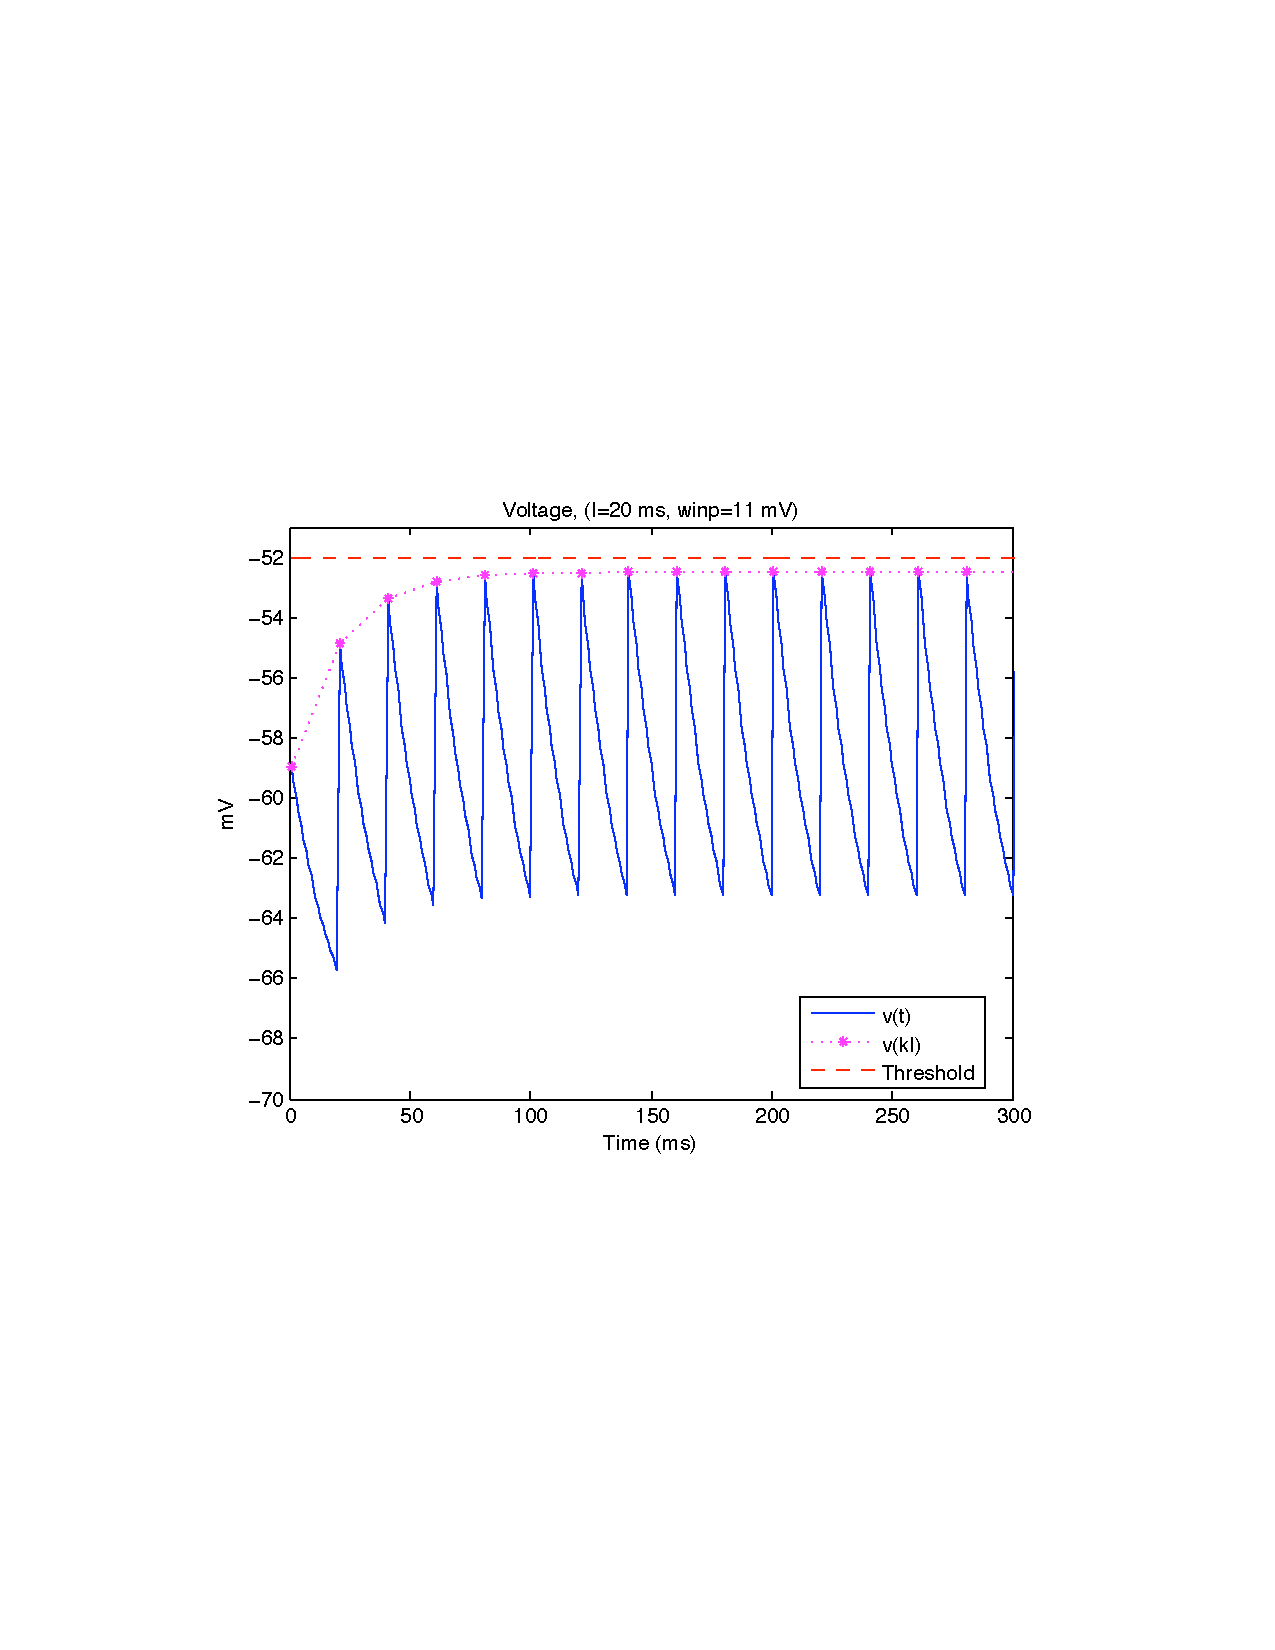
\includegraphics[scale=0.75]{AnpeakV.pdf}
\caption{Voltage as a function of time as calculated by equation \eqref{eq:anvinp}. The peak voltages are denoted by asterisks. Here we set $v_{th}=-52\ mV$. (\textbf{AnpeakV.m})}
\end{center}
\end{figure}

\section{Problems and Results}
\subsection{Minimum input weight for activity}
\label{seq:minw}

\subsubsection{Computational vs. Analytic Method}
We found the minimum input weight $w_{inp}$ necessary for the cell to spike at least once as a function of the input time interval $I$ when given a sufficiently long simulation.

Let the interspike interval $I$ and input weights $w_{inp}$ satisfy $2\leq I\leq 30$ and $2\leq w_{inp}\leq 20$.

In the computational method, the Matlab program \textbf{compW.m} calculates $v(t)$ according to equations \eqref{eq:compvbtwn} and \eqref{eq:compvinp}. In \textbf{AnalysisW.m}, the minimum $w_{inp}$ is calculated by
\begin{equation}
w_{inp} = (v_{th}-v_r)(1 - e^{-I/\tau}),
\label{eq:wanalysis}
\end{equation}
which was obtained by setting $v_\infty$ of equation \eqref{eq:Vasymp} to $v_\infty\geq v_{th}$ where
$$v_{th}\leq v_r + w_{inp}\left(\frac{1}{1-e^{-I/\tau}}\right).$$

Figure \ref{fig:BothWinpsxI} shows that as the input time interval increases, greater input weight is necessary for the cell to spike at least once (\textbf{AnalysisW.m}). We note on the graph the value of $w_{inp}=10.11$ at $I=20$ because these two values will be put to use in the next section.

\begin{figure}
\begin{center}
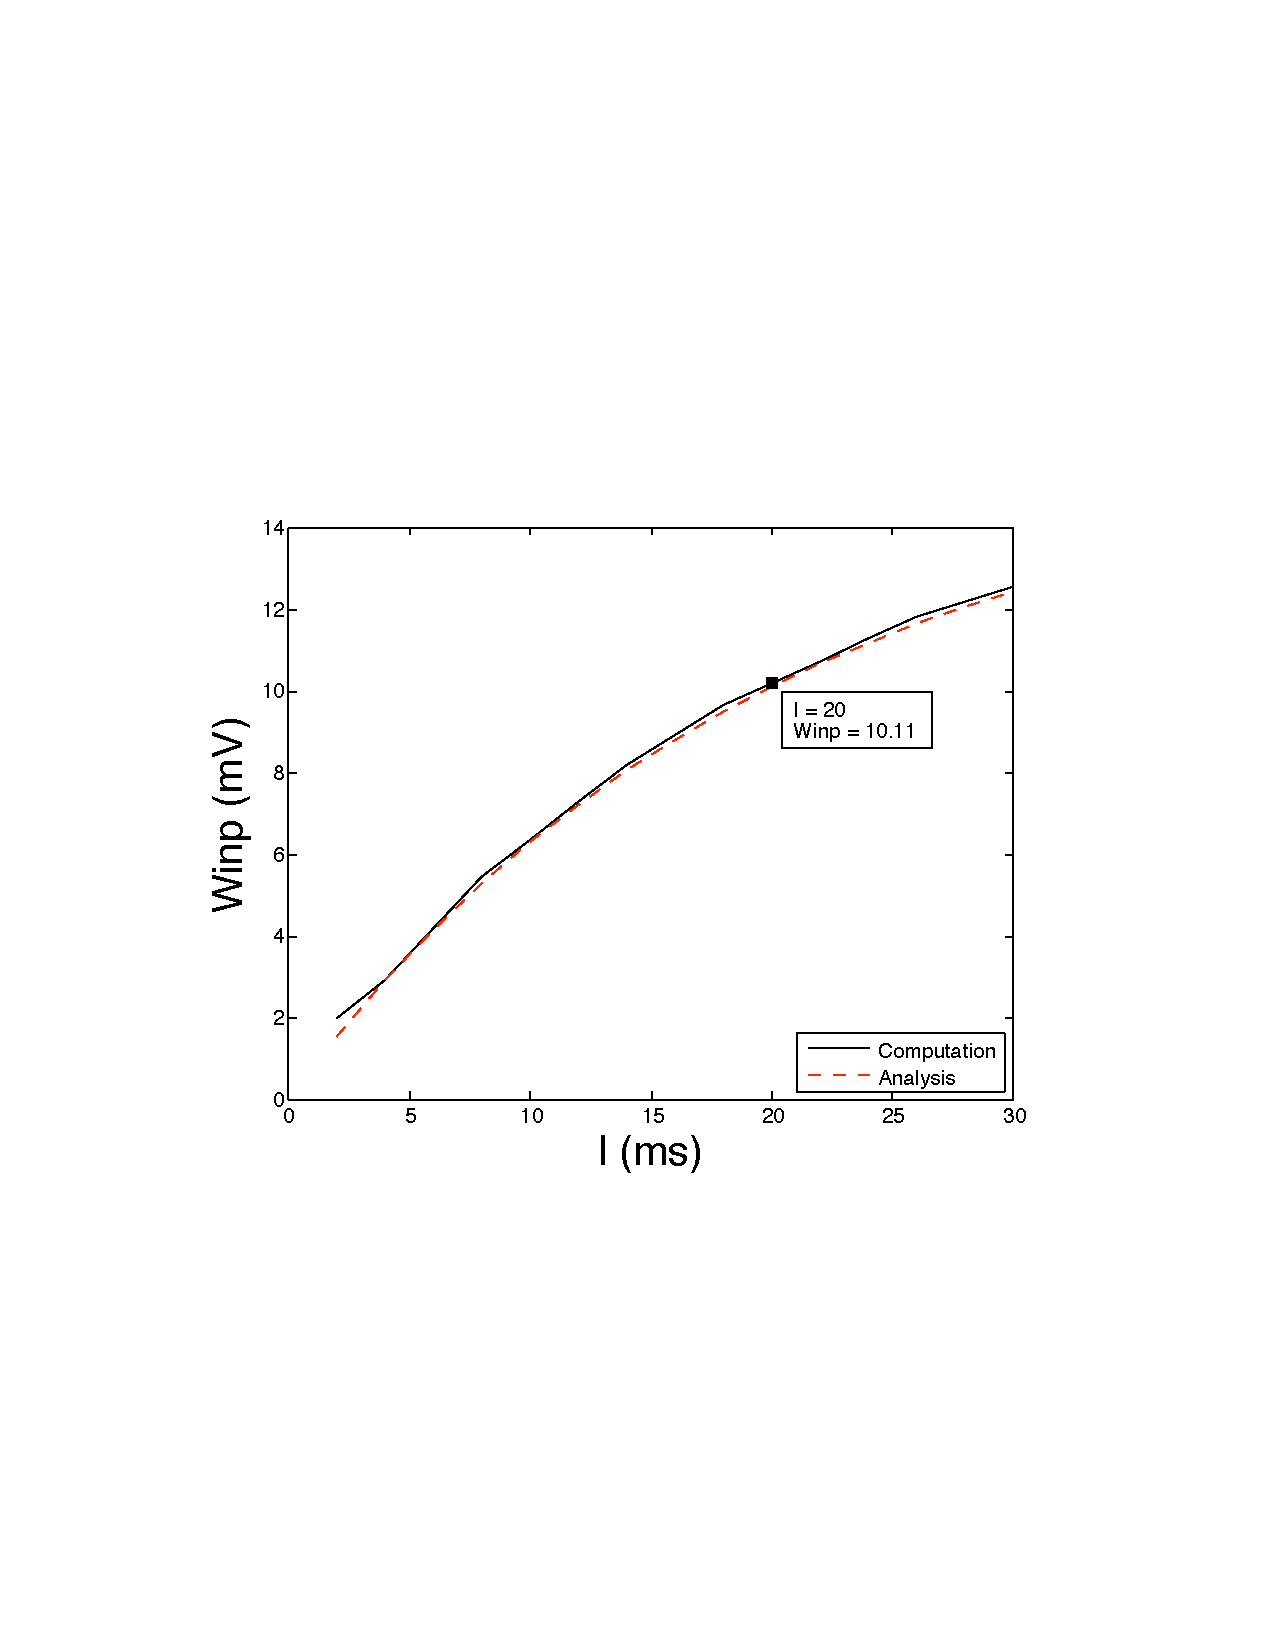
\includegraphics[scale=0.75]{BothWinpsxI.pdf}
\caption{Comparison of $w_{inp}$ from computation and analysis as a function of $I$. $v(t)$ is calculated by equations \eqref{eq:compvbtwn} and \eqref{eq:compvinp} in \textbf{compW.m}. $w_{inp}$ is calculated by equation \eqref{eq:wanalysis} in \textbf{AnalysisW.m}. (Plotted in \textbf{AnalysisW.m})}
\label{fig:BothWinpsxI}
\end{center}
\end{figure}

\subsection{Number of input spikes versus input weight}
\label{seq:firstspkt}

\subsubsection{Computational vs. Analytic Method}
We determine the minimum number of input spikes necessary for the cell to spike as a function of input weight.

We use $I=20$ and consider only the weights that produce at least one spike with sufficient simulation, starting with $w_{inp}=10.2$ as shown in Figure \ref{fig:BothWinpsxI}. Let $n_1$ denote the minimum number of input spikes of weight $w_{inp}$ necessary for $v(t)$ to reach $v_{th}$. We see that
\begin{equation}
n_1 \geq -\frac{\tau}{I}\cdot \ln \left( 1- \frac{v_{th}-v_r}{w_{inp}} \cdot\left(1-e^{-I/\tau}\right)\right).
\label{eq:n1analysis}
\end{equation}
In the computational method, the Matlab program \textbf{compT.m} calculates $n_1$ by updating $v(t)$ with equations \eqref{eq:compvbtwn} and \eqref{eq:compvinp}. In the analytic method, \textbf{AnalysisT.m} calculates $n_1$ with equation \eqref{eq:n1analysis}. 

% eqn for time of first spk as a function of winp
%For $0\leq k\leq n-1$ where $n$ is the total number of input spikes,
%$$t_1(w_{inp})=\min_{k\in\mathbb{N}} \{kI:v(kI)\geq v_{th}\},\quad \text{where }\mathbb{N}=\text{nonnegative integers}.$$ 
%where $v(kI)= v_r + w_{inp} \sum_{a=0}^{k} \left(e^{-I/\tau}\right)^k$ (equation \eqref{eq:anvinp}).

Figure \ref{fig:BothNinpxWinp} shows that $n_1$ is clearly a step-wise function where higher input weights allow the cell to spike after fewer input spikes. % reference .m files

%\begin{figure}
%\includegraphics[scale=0.75]{BothTxWinp.pdf}
%\caption{Comparison of $T_1$ from computation and analysis as a function of $w_{inp}$. $v(t)$ is calculated by equations \eqref{eq:compvbtwn} and \eqref{eq:compvinp} in \textbf{compT.m} and by equation \eqref{eq:anvinp} in \textbf{analysisT.m} .}
%\label{fig:BothTxWinp}
%\end{figure}

\begin{figure}
\begin{center}
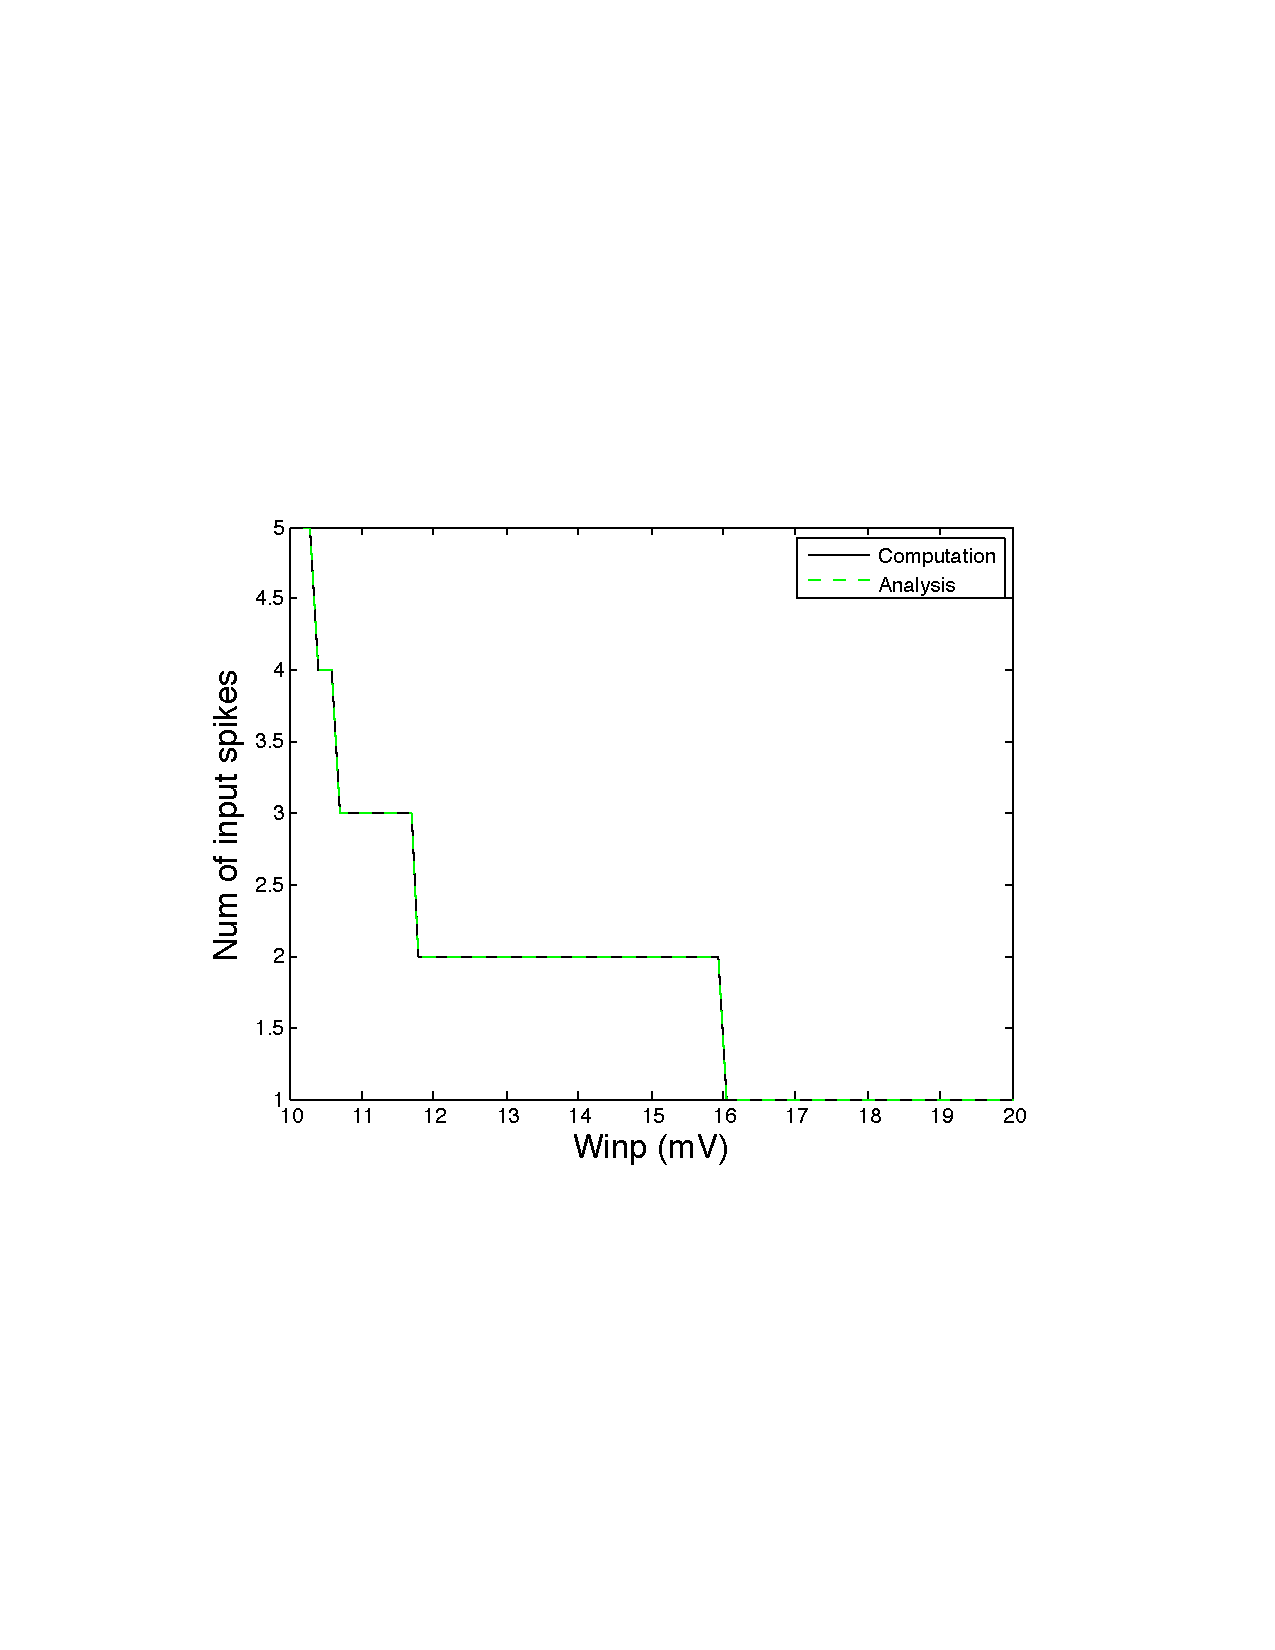
\includegraphics[scale=0.75]{BothNinpxWinp.pdf}
\caption{Comparison of minimum number of input spikes necessary for activity from computation and analysis as a function of $w_{inp}$. $v(t)$ is calculated by equations \eqref{eq:compvbtwn} and \eqref{eq:compvinp} in \textbf{compT.m} and by equation \eqref{eq:anvinp} in \textbf{AnalysisT.m}. (Plotted in \textbf{AnalysisT.m})}
\label{fig:BothNinpxWinp}
\end{center}
\end{figure}

\section{Application of findings}
\label{seq:apps}
\begin{figure}
\begin{center}
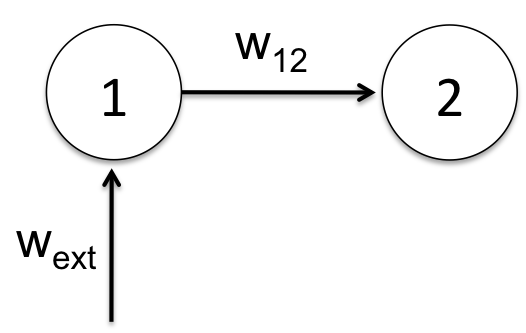
\includegraphics[scale=0.75]{PF1-2cells}
\caption{Simple 2-cell network with synapses active in Place Field 1. While the rat is in the place field of Cell 1, Cell 1 receives input with weight $w_{ext}$ from an external source, and when Cell 1 spikes, it gives input with weight $w_{12}$ to Cell 2.}
\label{fig:2cellsPF1}
\end{center}
\end{figure}

We apply the results from the two previous sections to solve a couple simple questions. Consider the situation depicted in Figure \ref{fig:2cellsPF1}: the rat is in Place Field 1, Cell 1 receives input with weight $w_{ext}$ from an external source, and, when Cell 1 spikes, it gives internal input to Cell 2 with weight $w_{12}$. We can find the minimum weight of $w_{12}$ necessary for Cell 2 to spike in Place Field 1, or where Place Field 1 and Place Field 2 overlap.

For a fixed interspike interval $I$ of external input of fixed weight $w_{ext}$, we calculate $n_1$ using equation \eqref{eq:n1analysis} as a function of $I$ and $w_{ext}$. Thus $n_1$ denotes the minimum number of external input spikes of weight $w_{ext}$ necessary for Cell 1 to fire. Let us denote the time of Cell 1's first spike as
$$t_1 = (n_1-1)I.$$

While the rat is in Place Field 1, Cell 2 only receives input from Cell 1. To find the interspike interval of Cell 1's spikes, or equivalently the interspike interval that Cell 2 receives input in Place Field 1, consider Figure \ref{fig:cell1spkfreq}. We know that Cell 1's first spike is at $t=t_1$. After it spikes, the voltage decays until the next input spike at $n_1 I$. Then it takes another $(n_1-1)I\ ms$ for Cell 1 to spike at $t=n_1 I + (n_1-1)I$. Thus we subtract the first spike time from the second spike time
$$n_1 I + (n_1-1)I-(n_1-1)I=n_1 I,$$
and we see that after the first spike time at $t_1=(n_1-1)I\ ms$, Cell 1 fires every $n_1 I \ ms$. 

\begin{figure}
\begin{center}

\includegraphics[scale=0.45]{cell1spkfreq}
\caption{Interspike interval of Cell 1 from external input alone, $I_1$. Cell 1's first spike occurs at $t=t_1=(n_1-1)I$. Then the voltage of Cell 1 decays until the next input spike at $t=n_1 I$. It then takes another $(n_1-1)I\ ms$ for Cell 1 to spike at $t=n_1 I + (n_1-1)I$. Thus, it can be seen that except for the first spike at $t=(n_1 -1)I$, Cell 1 fires every $n_1 I\ ms$.}
\label{fig:cell1spkfreq}
\end{center}
\end{figure}

Thus, we know that Cell 1 gives input to Cell 2 with weight $w_{12}$ every $n_1 I\ ms$. 
To find the minimum weight of $w_{12}$ that would allow for Cell 2 to fire in Place Field 1, we consider two cases where the first is simpler: Place Field 1 is infinitely long or finitely long.

Equation \eqref{eq:wanalysis} tells us that if
\begin{equation}
\label{eq:w12}
w_{12}\geq (v_{th}-v_r)(1-e^{-n_1 I/\tau}),
\end{equation}
then Cell 2 would fire given a sufficiently long Place Field 1. Thus, if Place Field 1 is infinitely long, we simply require that equation \eqref{eq:w12} be true, then Cell 2 fires in Place Field 1. As we do in Section \ref{seq:firstspkt}, we choose an interspike interval: let $n_1 I=40\ ms$. For this value of $n_1 I$, \textbf{App.m} calculates the minimum of equation \eqref{eq:w12} to be $13.83\ mV$, as marked in Figure \ref{fig:w12xn1I}.

\begin{figure}
\begin{center}
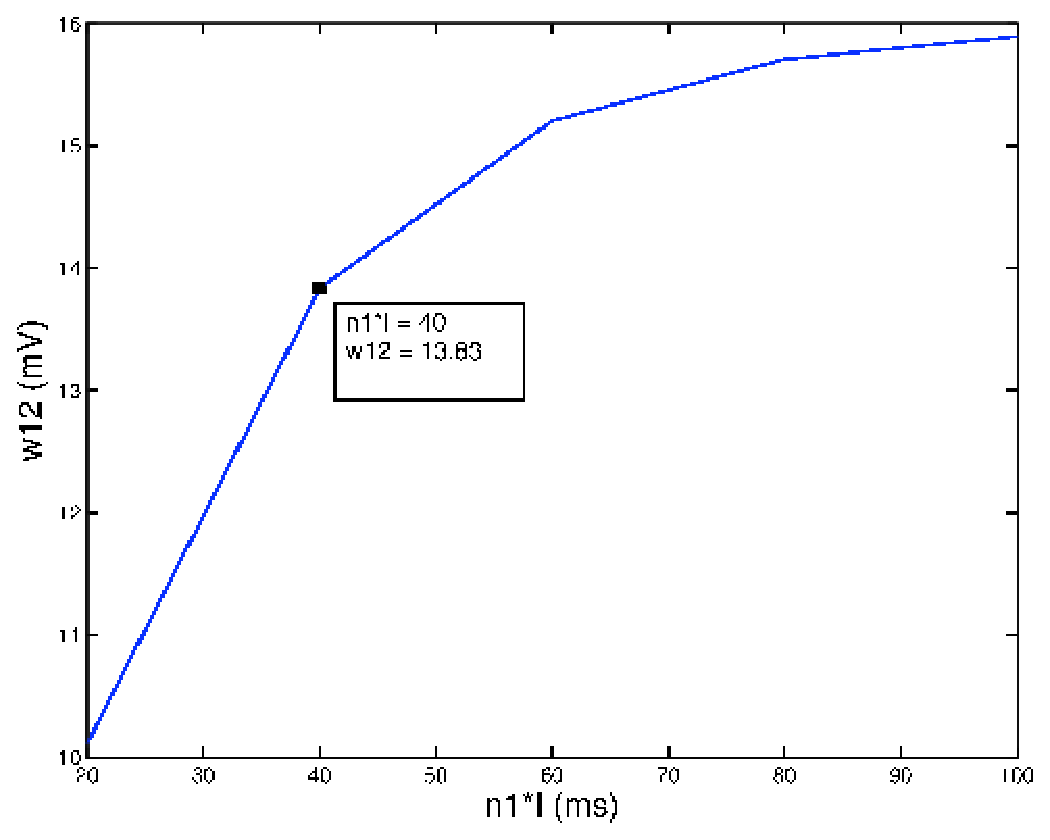
\includegraphics[scale=0.65]{w12xn1I}
\caption{Minimum $w_{12}$ necessary for Cell 2 to fire as a function of $n_1 I$. It is clear that the larger the interspike interval, the more weight is required for activity. We note the value of $w_{12}$ at $n_1 I=40$ because these values are used in the case where Place Field 1 is finite. (\textbf{App.m})}
\label{fig:w12xn1I}
\end{center}
\end{figure}

Now assume Place Field 1 is finitely long. 
We apply equation \eqref{eq:n1analysis} to find $n_2$, where $n_2$ is the minimum number of input spikes of weight $w_{12}$ necessary for Cell 2 to fire. We let $n_1 I=40\ ms$ and consider only the values of $w_{12}\geq 13.83\ mV$ as calculated for $n_1 I=40\ mV$ in equation \eqref{eq:w12}. Figure \ref{fig:n2xw12} shows $n_2$ as a function of these values of $w_{12}$. As in Section \ref{seq:firstspkt}, $n_2$ is step-wise like $n_1$.

\begin{figure}
\begin{center}
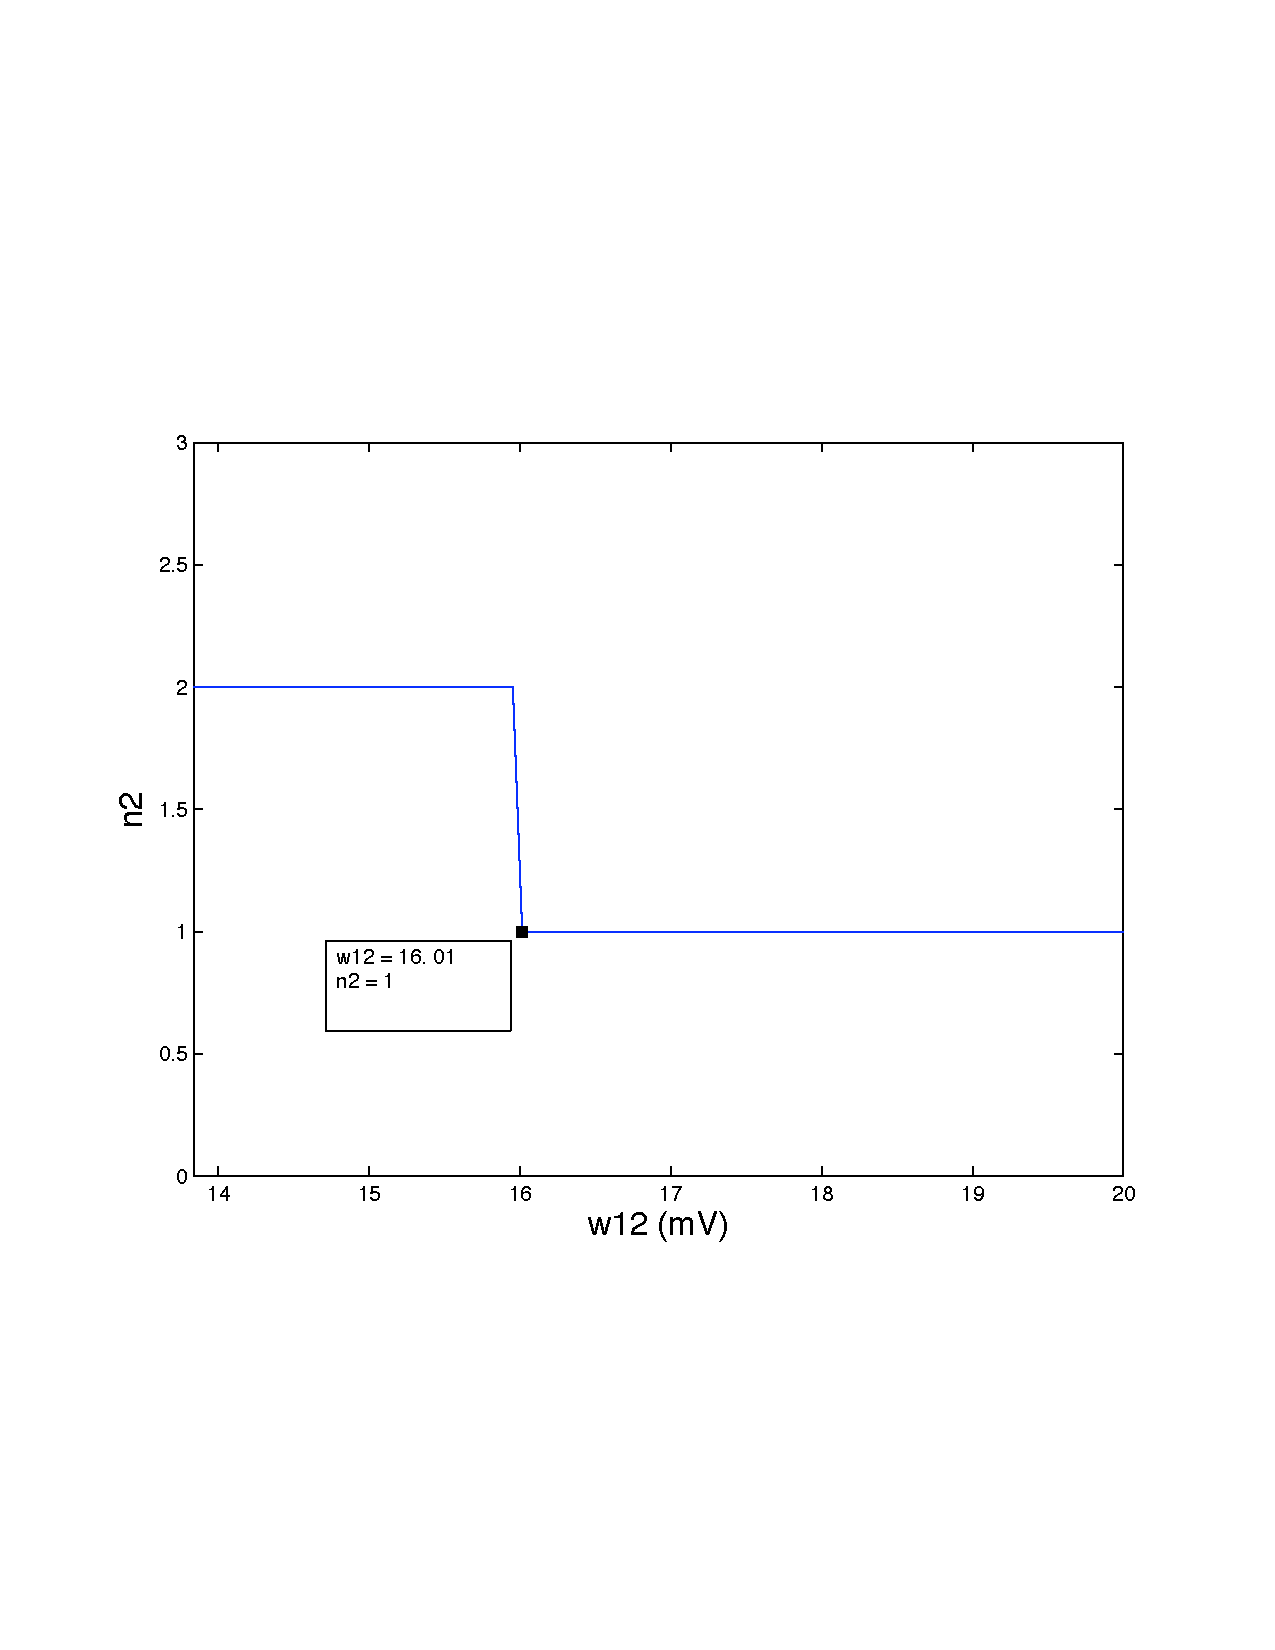
\includegraphics[scale=0.65]{n2xw12}
\caption{Minimum number of input spikes necessary for Cell 2 to fire, denoted as $n_2$, as a function of input weight $w_{12}$. We choose $n_1 I = 40\ ms$ and consider only the values of $w_{12}\geq 13.83\ mV$ (the minimum $w_{12}$ necessary for Cell 1 to fire from equation \eqref{eq:w12}). Like $n_1$ from Section \ref{seq:firstspkt}, $n_2$ is step-wise. We note the minimum weight necessary for Cell 2 to fire in Place Field 1, $w_{12}=16.01\ mV$. (\textbf{App.m})}
\label{fig:n2xw12}
\end{center}
\end{figure}

The first spike of Cell 2 occurs at time $t_2=(n_2)(n_1 I)-I$. We find the value of $w_{12}$ necessary for $t_2\leq$ the time spent in Place Field 1. Suppose the time spent in Place Field 1 is $50\ ms$. We see from Figure \ref{fig:n2xw12} that
$$n_2= \left\{
\begin{array}{ll}
	2 & \text{ if } 13.83\leq w_{12}\leq 15.95\\
	1 & \text{ if } 15.95< w_{12}\leq 20.00
\end{array}
\right.$$
and calculate that
$$t_2= \left\{
\begin{array}{ll}
	60 & \text{ if } 13.83\leq w_{12}\leq 15.95\\
	20 & \text{ if } 15.95< w_{12}\leq 20.00
\end{array}
\right.$$
Thus, for $13.83\leq w_{12}\leq 15.95\ mV$, $t_2=60\ ms$ and Cell 2 will not fire in Place Field 1, but for $16.01\leq w_{12}\leq 20.00\ mV$, $t_2=20\ ms$ and Cell 2 will fire in Place Field 1.
The minimum value of $w_{12}$ for $t_2 \leq 50\ ms$ is marked on Figure \ref{fig:n2xw12} (\textbf{App.m}).

\section{Future work}

Our goal is to better understand the relation between input weights and backward shift of place fields. We modeled the Double Rotation Experiment using a simple 120-cell ring and calculated the backward shift of the place fields as a function of input weights of that model \cite{KnierimDRE,Cox}.
We have computationally and analytically found the minimum input weight necessary for activity as a function of the interspike interval as well as the minimum number of input spikes necessary for activity as a function of input weight.
We applied our findings analytically to find the minimum internal input weight necessary for place fields to overlap in a simple 2-cell model.

Future work may include constructing a code to compare our analytical results from Section \ref{seq:apps} for the infinite and finite place field cases that could give us the minimum internal input weight necessary for place fields to overlap. We could also couple the equations regarding input weight changes by spike timing-dependent plasticity with the equation that gives us the minimum number of input spikes necessary for activity that is dependent upon input weights. Since the time of the first spike of a cell can be given in terms of the minimum number of input spikes necessary for activity as a function of input weight, we may be able to find a value that the time approaches. Ultimately, given a set maximum for the input weight, we would like to be able to predict the amount of backward shift of a place field using spike timing-dependent plasticity.

%-------------------------------------------------------------------
% to create references, un-comment \bibliographystyle{plain} and
% un-comment \bibliography{myBIBfile} and re-name its argument(s)
% to point at the .bib file(s) containing the BibTeX references:

\bibliographystyle{plain}
\bibliography{Writeup2}


\end{document}
